\chapter{Sistema proposto}
\label{cap:sistema_proposto}

\section{Introdução}

\section{Arquitetura}

Essa seção descreve a arquitetura do sistema através de duas modelagens: lógica e física. A primeira apresenta os componentes abstraindo as tecnologias envolvidas na sua composição. Já o modelo complementa a visão lógica a partir do detalhamento da implementação dos componentes bem como as tecnologias empregadas em suas respectivas implementações.

\subsection{Modelo lógico}

O modelo lógico do sistema proposto neste trabalho é apresentado na Figura \ref{fig:c4_modelo_logico}. Pode-se observar, portanto, quatro camadas: aplicação, serviços, repositórios e processamento. A primeira delas, de aplicação, envolve todos os agentes externos ao servidor principal, sendo eles, geladeira, interface de usuário e o mercado. Já as demais, de serviços, repositórios e processamento se encontram dentro do servidor sendo estas separadas por módulos.

% Figura

% Explicar figura
% Explicação das camadas
\begin{figure}[htb]
    \caption{Modelo lógico}
    \label{fig:c4_modelo_logico}
    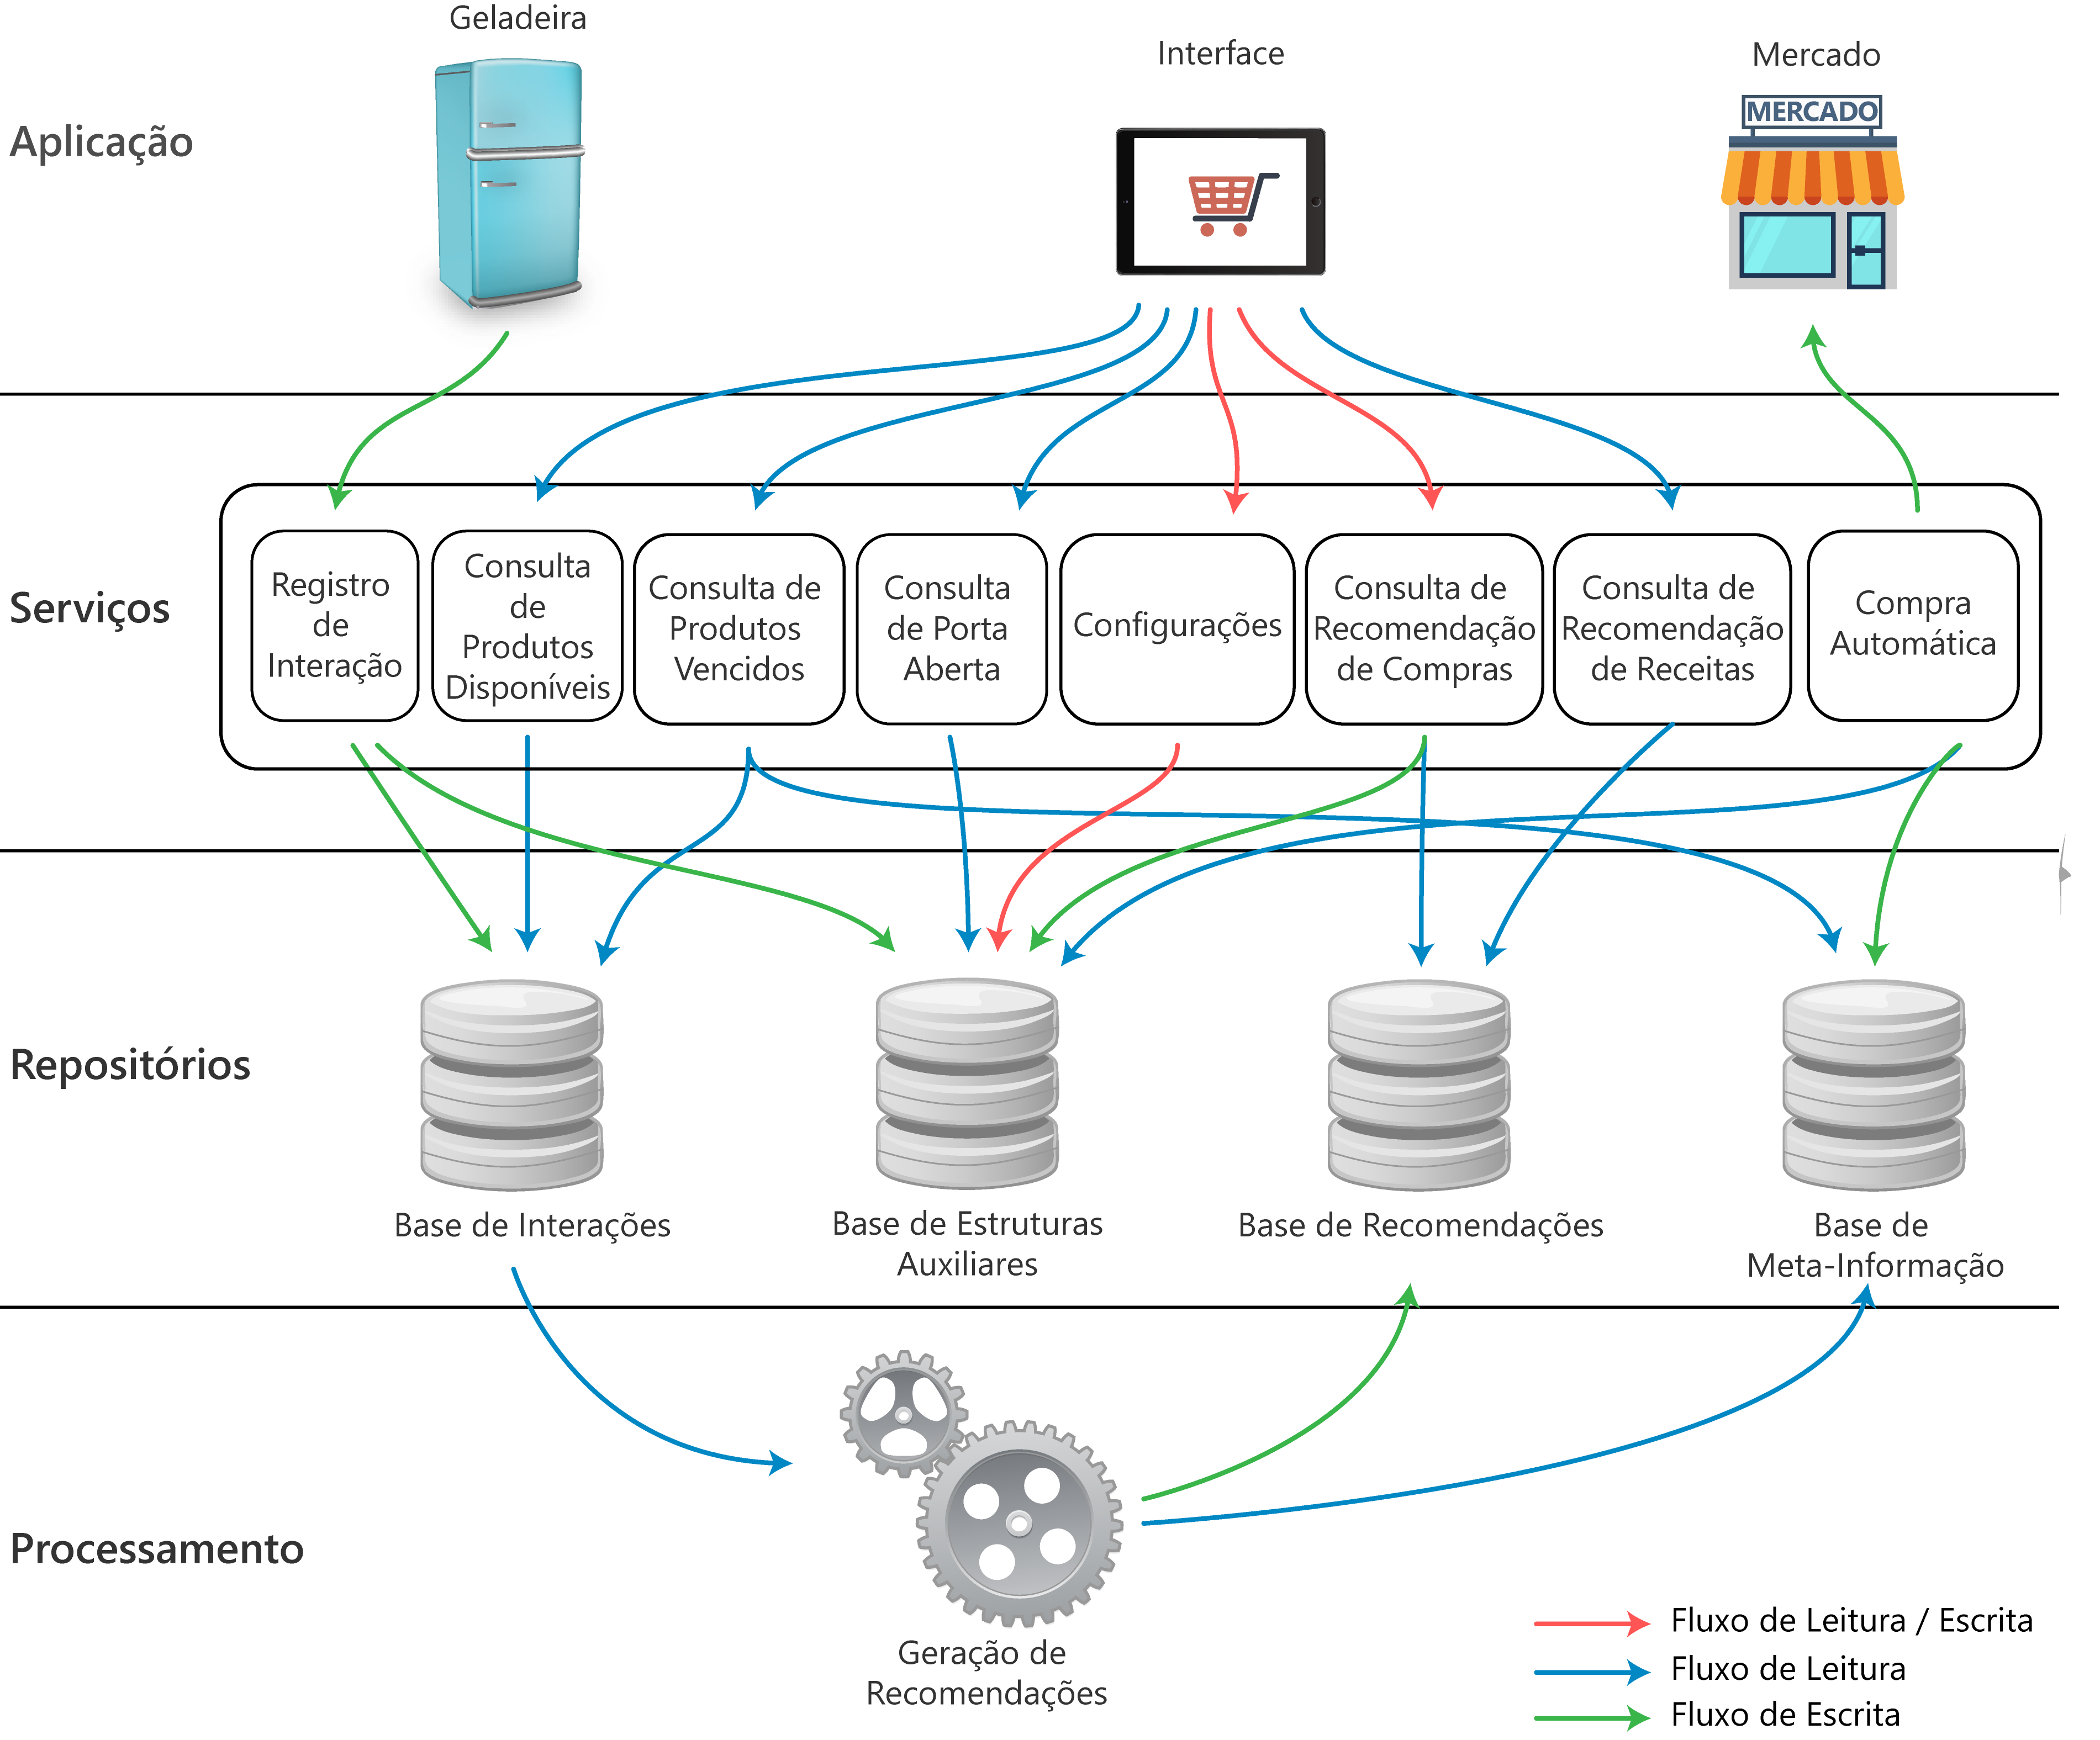
\includegraphics[width=\textwidth]{modelo-logico}
    
    Fonte: Autores
\end{figure}
\nocite{Freepik2017} % fonte dos ícones

\subsubsection{Camada de Aplicação}

% Explanação sobre a camada

% Descrição da geladeira
%  - O que é
%  - Qual objetivo
%  - Porque

A camada de aplicação, como já dito, envolve os agentes externos. O primeiro deles é a geladeira à qual é responsável por monitorar os produtos nela contidos. Deste modo, a cada interação do usuário com a geladeira, esta fará uma varredura para verificar o conjunto de produtos existentes. Em seguida, enviará tais informações para o servidor através do serviço de registro de interação. Além disso, a geladeira também é responsável por verificar a condição de fechamento porta e, caso aberta, a geladeira fará um registro através do serviço de estruturas auxiliares para que o sistema seja capaz de emitir um aviso ao usuário.

% Descrição da interface
%  - O que é
%  - Qual objetivo
%  - Porque

O componente seguinte é a interface de usuário que é incorporada à porta da geladeira e que responsabiliza-se por permitir ao usuário a interação com o eletrodoméstico. A partir disso, tem-se como funcionalidades deste componente, a listagem de produtos contidos, produtos com prazos de validade próximos, avisos de porta aberta, configurações e, por fim, recomendações de possíveis compras de produtos e receitas.

% Descrição do mercado
%  - O que é
%  - Qual objetivo
%  - Porque

%O último componente da camada de aplicação é o mercado. 
%A partir deste será possível fazer verificações da existência de produtos da geladeira com prazo de validade expirados. 
%Além disso, permite que, 
O último componente é o mercado. Através dele, será possível efetivar as compras a partir da lista de produtos selecionada pelo usuário dentre os recomendados. Além disso, é possível fazer consultas de promoções de itens que eventualmente serão disponibilizadas pelo mercado. Por fim, esse componente pode ser interpretado como outro sistema que apresenta seus respectivos serviços e repositórios.

\subsubsection{Camada de Serviços}

A camada de serviços disponibiliza um conjunto de funcionalidades aos componentes da camada de aplicação se comportando como intermediadora entre aplicação com o sistema principal. Assim, há um conjunto de serviços específicos disponibilizados conforme a Figura \ref{fig:c4_modelo_logico} e que serão descritos nos parágrafos seguintes.

% Explanação sobre a camada serviços

% Descrição do "Registro de interação"
%  - O que é
%  - Qual objetivo
%  - Porque
O serviço de registro de interação receberá informações dos itens contidos da geladeira além do alerta de porta aberta. Em seguida, registra-se tais informações na base de interações e de estruturas auxiliares, respectivamente.


% Descrição do "Consulta de Produtos Disponíveis"
%  - O que é
%  - Qual objetivo
%  - Porque

Já o serviço de consulta de produtos disponíveis será requisitado pelo usuário através da interface. Então, será feita uma busca na base de interações pelo último registro feito ao qual conterá os produtos existentes.

% Descrição do "Consulta de produtos vencidos"
%  - O que é
%  - Qual objetivo
%  - Porque

O serviço de consulta de produtos vencidos é realizada periodicamente pela interface. Desse modo, é feita uma busca pelo itens disponíveis na geladeira e o tempo que estão presentes através da base de interações. Logo após, é feita uma consulta na base de meta-informação para determinar o tempo estimado de validade de cada produto encontrado. A partir da comparação entre tempo de acondicionamento e prazo de expiração, sabe-se se o produto está vencido ou não. A estimativa é feita pois o prazo de validade transcrito em produtos não condiz após a abertura do produto. Assim, uma estimativa de tempo menor é necessária.

% Descrição do "Consulta de porta aberta"
%  - O que é
%  - Qual objetivo
%  - Porque
O serviço de consulta de porta aberta é requisitado pela interface de usuário periodicamente de forma automática. Como efeito da requisição, faz-se uma consulta à base de estruturas auxiliares a fim verificar a existência de um registro recente de porta aberta. O resultado é então encaminhado para a interface que alertará o usuário, caso necessário.

% TODO: O último registro diz se a porta está aberta ou não.

% Descrição do "Configurações"
%  - O que é
%  - Qual objetivo
%  - Porque

O serviço de configurações permite que o usuário personalize algumas características do funcionamento da geladeira. A primeira delas se refere ao mercado no qual as compras são realizadas. 

% Descrição do "Consulta de Recomendação de Compras"
%  - O que é
%  - Qual objetivo
%  - Porque

O serviço de consulta de recomendação de compras é requisitado pela aplicação periodicamente. Assim, quando é feita uma requisição, o serviço faz uma consulta à base de recomendações em busca de possíveis sugestões. O conjunto existente é então retornado para a interface que, por sua vez, indaga ao usuário se deseja realizar a compra e quais produtos deseja adquirir, dentre os apresentados. A lista é retornada ao serviço que, então, faz o registro na base de estruturas auxiliares.

% Descrição do "Consulta de Recomendação de Receitas"
%  - O que é
%  - Qual objetivo
%  - Porque

O serviço de recomendação de receitas recebe uma requisição do usuário e faz uma consulta à base de recomendações. Caso existam receitas para recomendar, essas serão listadas ao usuário na interface e será possível então a escolha de qual receita deseja-se visualizar.

% Descrição do "Compra automática"
%  - O que é
%  - Qual objetivo
%  - Porque

O serviço de compra automática é executado automaticamente quando há uma lista de compras pendente. Assim, a partir da verificação de tal pendência na base de estruturas auxiliares, a compra é requisitada ao agente mercado e como retorno, informações a cerca das características dos produtos serão retornadas e gravadas na base de meta-informação para uso posterior pelo mecanismo gerador de recomendação. 

\subsubsection{Camada de Repositórios}

% Explanação sobre a camada
O conjunto de repositórios desta camada atuam na persistência de informações geradas pelos diversos componentes e pelo gerador de recomendação. Nessa modelagem, dividiu-se em quatro bases: de interações, de estruturas auxiliares, de recomendações e de meta-informação.
A primeira base é responsável, como descrito anteriormente, pelo registro de produtos acondicionados na geladeira. A partir disso, as consultas realizadas nessa base recuperarão os itens constantes após cada interação do usuário.

A base de estruturas auxiliares contém informações que são utilizadas por mais de um serviço. Tais informações são alertas de porta aberta, configurações e as listas de compras determinadas pelo usuário. 

Já a base de recomendações armazena todas as sugestões de receitas e de compras construídas pelo gerador e que serão apresentadas ao usuário.

A última base, de meta-informação contém informações referentes ao conteúdo dos produtos adquiridos e que são utilizadas pelo gerador de recomendações e pelo serviço de verificação de produtos vencidos. Tais informações incluem características do produto bem como tempo estimado de validade.

\subsubsection{Camada de Processamento}

% Explanação sobre a camada
A camada de processamento contém o módulo de geração de recomendações. Tal componente faz uso das informações armazenadas na base de interação e das características de cada item mantidas na base de meta-informações.

% Como vai receber do mercado informações de que tem itens em promoção.
As recomendações de receitas fazem uso da base de interações para ter conhecimento dos produtos contidos atualmente e de meta-informações para resgatar as receitas e seus respectivos ingredientes. A partir disso, é feita uma comparação entre as bases. Caso alguma receita requeira itens que já estão presentes, essa será recomendada ao usuário. Do contrário, caso apenas alguns poucos itens estejam em falta, será sugerida, ao usuário, além da receita, a compra de tais produtos faltantes.

Compras são sugeridas com base na quantidade existente de um certo produto. Assim, quando tal valor cai abaixo da quantidade mínima, determinada pelo usuário, é feita a recomendação de compra do mesmo item. No entanto, o mercado pode não ter à disposição o produto específico, mas pode conter similares. Nesse caso, o sistema faz uma busca por itens similares e pede a aprovação do usuário para a compra do item semelhante, ao invés do original. Além disso, sugere-se novos itens com base em promoções que por ventura o mercado venha a disponibilizar e que o usuário tenha apresentado interesse em tais produtos.

\subsection{Modelo físico}
% Descrição da geladeira
%  - O que é
%  - Qual objetivo
%  - Porque

% Explicar o que há dentro de cada componente lógico
% Se preciso desenhar a arquitetura interna do componente
% Por exemplo a geladeira, vai ter muitas coisas dentro que devem ser explicitadas

\subsection{Exemplo de fluxo de execução}